% Note to reader: lines beginning with the '%' character are
% 'comments' to you, the human reader of this code, and are 
% ignored by the LaTeX compiler.

%%%%%%%%%%%%%%%%%%%%%%%%%%%%%%%%%%%%%%%%%%%%%%%%%%%%%%%%%%%%%%%%%%
% = Sample template for MIT Junior Lab Student Written Summaries =
% Available from 
%    http://web.mit.edu/8.13/www/Samplepaper/sample-paper.tex
%
% Last Updated July 23, 2014
%
% Adapted from the American Physical Societies REVTeK-4.1 Pages
%    at http://publish.aps.org
%
% ADVICE TO STUDENTS: Each time you write a paper, start with this
%    template and save under a new filename.  If convenient, don't
%    erase unneeded lines, just comment them out using the 
%    '%' character at the start of the line.  Often, they
%    will be useful containers for information.
%
% Using pdflatex, images must be either PNG, GIF, JPEG or PDF.
%    Turn EPS (encapsulated postscript) images to PDF using the
%    epstopdf utility on UNIX systems.
%%%%%%%%%%%%%%%%%%%%%%%%%%%%%%%%%%%%%%%%%%%%%%%%%%%%%%%%%%%%%%%%%%

%%%%%%%%%%%%%%%%%%%%%%%%%%%%%%%%%%%%%%%%%%%%%%%%%%%%%%%%%%%%%%%%%%
% = TO COMPILE THIS DOCUMENT =
%
% From the command line, it would go like this --- assuming you are
%    in the directory where the filename.tex source file and the 
%    filename.bib bibliography file are located, and that you have 
%    permission to create and write files in that directory:
%      > pdflatex filename
%      > bibtex filename
%      > pdflatex filname
%      > pdflatex filename
%    Yes, you run the command several times. The earlier runs 
%    create auxilliary files which keep track of references,
%    citations, equation and section numberring, etc. The later
%    runs combine the information in these auxilliary files with
%    your source document to create the finished product.
%
% If you are using a GUI LaTeX editor like TeXWorks, then there
%    is probably a menu bar button for pdfLaTeX and another for
%    BibTeX. Hit them in the order indicated above. There is 
%    probably also a 'TeXify' button, or something similarly named,
%    which runs all the above commands in one shot.     
%%%%%%%%%%%%%%%%%%%%%%%%%%%%%%%%%%%%%%%%%%%%%%%%%%%%%%%%%%%%%%%%%%


%%%%%%%%%%%%%%%%%%%%%%%%%%%%%%%%%%%%%%%%%%%%%%%%%%%%%%%%%%%%%%%%%%
%  = PREAMBLE =
% The preamble of a LaTeX document is the set of commands that precede
% the \begin{document} line.  It contains a \documentclass line
% to load the REVTeK-4.1 macro definitions and various \usepackage
% lines to load other macro packages.
%
% ADVICE TO STUDENTS: This preamble contains a suggested set of
%     class options to generate a ``Junior Lab'' look and feel that
%     facilitate quick review and feedback from one's peers, TAs,
%     and section instructors.  Don't make substantial changes 
%     to the style without first consulting your section 
%     instructor.
%%%%%%%%%%%%%%%%%%%%%%%%%%%%%%%%%%%%%%%%%%%%%%%%%%%%%%%%%%%%%%%%%%

%\documentclass[aps,twocolumn,secnumarabic,balancelastpage,amsmath,amssymb,nofootinbib, floatfix]{revtex4}
\documentclass[aps,twocolumn,nobalancelastpage,secnumarabic,amsmath,amssymb,nofootinbib,floatfix]{revtex4-1}

%%%%%%%%%%%%%%%%%%%%%%%%%%%%%%%%%%%%%%%%%%%%%%%%%%%%%%%%%%%%%%%%%%%
% N.B.:  Different computers have different packages installed.  
%        To compile this template in the current Athena 
%        environment, REVTeX 4.1 must be used.  To use the older
%        REVTeX 4, switch which documentclass line above is 
%        commented out above. There are ``bad'' distributions of
%        LaTeX for Windows available on the internet which may 
%        cause users to struggle unjustifiably with REVTeX 4.1.
%
%        If you are unable to compile the template at all, you
%        may need to update your LaTeX packages. (Alternatively, if 
%        your LaTeX distribution includes only the older RevTEX 4,
%        then try changing the documentclass line above. In particular,
%        this approach solves a common compilation problem for users of
%        the TeXWorks editor on Windows, which presents erroneously as a
%        error in the bibliography file.) Don't hesitate to speak 
%        with your section instructor or a TA if you're having 
%        issues getting this template to compile.
%%%%%%%%%%%%%%%%%%%%%%%%%%%%%%%%%%%%%%%%%%%%%%%%%%%%%%%%%%%%%%%%%%%

%%%%%%%%%%%%%%%%%%%%%%%%%%%%%%%%%%%%%%%%%%%%%%%%%%%%%%%%%%%%%%%%%%%
% = Explanation of documentclass options =
%
% aps, prl stand for American Physical Society and Physical 
%     Review Letters respectively.
% twocolumn permits two columns, of course.
% nobalancelastpage doesn't attempt to equalize the lengths of 
%     the two columns on the last page  as might be desired in a 
%     journal where articles follow one another closely.
% amsmath and amssymb are necessary for the subequations 
%     environment among others. These functionalities can
%     also be added use the usepackage function described below,
%     but REVTeX conveniently includes them as documentclass
%     options.
% secnumarabic identifies sections by number to aid electronic 
%     review and commentary.
% nofootinbib forces footnotes to occur on the page where they are
%      first referenced and not in the bibliography.
% floatfix attempts to help LaTeX decide where to place ``floats'',
%      like figures and plots, when it gets stuck and can't decide
%      by it's normal algorithm.
% REVTeX 4.1 is a set of macro packages designed to be used with 
%      LaTeX 2e. REVTeX is well-suited for preparing manuscripts 
%      for submission to APS journals.
%
% = Other documentclasses =
%
% The 'revtex4' and 'revtex4-1' documentclasses are somewhat 
%    specialized for making documents in the style of the APS
%    journals. For a more standard or generic looking LaTeX paper,
%    you could try any of the built-in documentclasses, in 
%    particular 'article' or 'report'. Someday, you may try to use 
%    the 'mitthesis'  documentclass available for download from the 
%    MIT Libraries. The vast majority of source code written for 
%    one documentclass should work just fine in any other, but 
%    occasional quirks arise. For example, some documentclasses 
%    disagree on whether the abstract declaration should come 
%    before or after the \begin{document} declaration.
% 
%%%%%%%%%%%%%%%%%%%%%%%%%%%%%%%%%%%%%%%%%%%%%%%%%%%%%%%%%%%%%%%%%%%

%% Now, include some packages which provide new commands that 
%% extend LaTeX's capabilities. Note that the nearly-essential
%% AMS math packages were added already as documentclass options
%% for REVTeX, but could have been added here using 
%% \usepackage{amsmath}, etc. The pacakges below are commonly 
%% useful, but there are many, many more available to solve a 
%% multitude of typesetting quandries (google your problem), 
%% and you  probably have the necesary packages installed on your
%% system already. Among the examples listed below, this sample
%% document only actually makes use of the 'graphicx', 'bm', 
%% and 'hyperref' pacakges, so the others are commented out for
%% tidyness.


\usepackage{graphicx}      % tools for importing graphics
\usepackage{lipsum}
\usepackage{float}
%\usepackage{lgrind}        % convert program code listings to a form 
                            % includable in a LaTeX document
%\usepackage{xcolor}        % produces boxes or entire pages with 
                            % colored backgrounds
%\usepackage{longtable}     % helps with long table options
%\usepackage{epsf}          % old package handles encapsulated postscript issues
\usepackage{bm}            % special bold-math package. usge: \bm{mathsymbol}
\usepackage{physics}
\usepackage{tensor}
\usepackage{gensymb}
%\usepackage{asymptote}     % For typesetting of mathematical illustrations
%\usepackage{thumbpdf}
\usepackage[colorlinks=true]{hyperref}  % this package should be added after 
                                        % all others.
                                        % usage: \url{http://web.mit.edu/8.13}


%%%%%%%%%%%%%%%%%%%%%%%%%%%%%%%%%%%%%%%%%%%%%%%%%%%%%%%%%%%%%%%%%%%
% And now, begin the document...
%%%%%%%%%%%%%%%%%%%%%%%%%%%%%%%%%%%%%%%%%%%%%%%%%%%%%%%%%%%%%%%%%%%

\begin{document}
\title{Galactic Structure Mapping through 21cm Hyperfine Hydrogen Transition Line}
\author{Henry Shackleton}
\email{hshackle@mit.edu}
\date{\today}
\affiliation{MIT Department of Physics}


\begin{abstract}
  Using a Small Radio Telescope (SRT), we measure electromagnetic radiation centered around 1420.4 MHz. This frequency corresponds to the hyperfine transition line in the hydrogen atom - a process so strongly forbidden that the only detectable sources of this transition are due to large galactic formations of hydrogen. By analyzing the Doppler shift in this 1420.4 MHz emission, we are able to determine the velocity of sections of the Milky Way galaxy. Futher geometric considerations allow us to determine the location of these high-density hydrogen structures, confirming a spiral-arm strucutre of the Milky Way galaxy.
\end{abstract}

\maketitle

\section{Introduction}
In 1944, Hendrick van de Hulst predicted an emission of 1420.4 MHz radiation from neutral hydrogen from a hyperfine splitting transition (detailed further in Section II). As electromagnetic energy in this range can pass through Earth's atmosphere easily, this discovery proved to be immensly useful in the field of astronomy. Soon after this discovery, Edward Purcell and Harold Ewen published a paper detailing their successful detection of this emission line through a radiometer. As hydrogen makes up 90\% of our galaxy's interstallar medium (ISM), a mapping of hydrogen density via this 21cm emission line can be used to extract details about the structure of our galaxy. In this paper, we reconstuct some of the key features of the Milky Way's spiral arm structure using radio astronomy.

\section{Theoretical Background}
Due to the low temperatures predominant in interstellar medium, hydrogen is most often found in its ground state. As a result of the intrinsic spins of both the proton and the electron, the hydrogen ground state has two modes - one where the two spins are aligned, and one where the spins oppose each other. These two states have an energy difference of $\Delta E = 5.884 \times 10^{-6}$ eV \cite{griffiths}, and when a hydrogen atom transitions from both spins being aligned to being disaligned, it emits radiation with a wavelength of 21cm, or with a frequency of 1420.4 MHz. This process is highly forbidden, occurring at a transition rate of $2.9 \times 10^{-15}\ s^{-1}$. However, the ISM is dense enough (1 atom per cubic centimeter) and large enough (on the order of kiloparsecs) to produce detectible amounts of radiation, which can be observed by a radio telescope. 

Because of the dynamic nature of our galaxy, hydrogen that we observe can be moving relative to us. This relative motion has a Doppler effect on the radiation frequency observed. The relationship between a body moving away from the Sun at a relative velocity $V$ and the frequency $f$ that we observe is given by
\begin{equation}
  V = \frac{(1420.406 - f)c}{1420.406} - V_{lsr}
\end{equation}
Where $c$ is the speed of light and $V_{lsr}$ corrects for the motion of the Earth around the Sun. The purpose of considering relative motion away from the Sun as opposed to the Earth is for the sake of geomoetric simplification.

\begin{figure}
  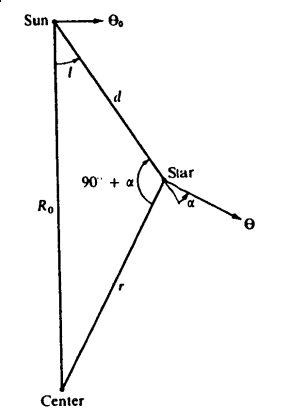
\includegraphics[width=0.3\textwidth]{geom}
  \caption{The relevant geometry of our galaxy, represented as a top-down view of the galactic disk. Known constants are the distance from our sun to the center of the galaxy,$R_0 = 8.2 \pm 0.5$ kpc, and the velocity of our sun. $\Theta_0 = 223 \pm 17$ km/s. The viewing angle $\ell$ is determined by the posiiton of our telescope.}
  \label{geom}
\end{figure}
Given this information, we can calculate the location of the hydrogen source through geometric considerations. Illustrated in Figure \ref{geom} is the relevant geometry of our galaxy. The velocity due to Doppler shifting is given by the $\textit{actual}$ velocity of the hydrogen mass $\Theta$ projected along the line of sight from the sun, minues the sun's velocity projected along the lihe of sight. Through the law of sines, we can calculate the general relation

\begin{equation}
  V &= \frac{\Theta}{r} R_0 \sin \ell - \Theta_0 \sin \ell
\end{equation}

Where $R_0$ and $r$ are the distances from the sun and our hydrogen mass to the center of the galaxy, $\Theta_0$ is the velocity of the sun, and $\ell$ is our viewing angle. Both $r$ and $\Theta$ are unknown, but a general relation between the radius of an object from the center of the galaxy and its velocity can be determined via the Galactic Rotation Curve. This gives an equation that allows us to calculate $r$ given the viewing angle $\ell$ and our observed velocity $V$. We restrict our viewing angle to $90\degree \leq \ell \leq 180\degree$. In this regime, the Galactic Rotation Curve predicts $\Theta$ to be approximately constant at $200$ km/s, which greatly simplifies calculations.



\section{Experimental Setup}
\subsection{Radio Telescope Specifications}
To detect radiation from these hyperfine transitions, we use a small radio telescope (SRT), capable of detecting and recording electromagnetic radiation. This telescope has a 7.5 foot diameter parabolic dish, and a beam width of approximately 7.0 degrees. This focal length will ultimately constrain the angular resolution of the data we collect. The telescope is controlled via a computer interface, a block diagram of which is detailed in Figure \ref{srt}. Radio signals are reflected off of the telescope's dish and into the antenna feed horn. In order to process this data, the signals are fed through a band pass filter, a low noise pre-amplifier, and a mixer. This converts our signal into a digital recording. As the bandwidth of our receiver is only approximately $0.5$ MHz, and is not wide enough to detect the degree of Doppler shifting necessary for this experiment, we use a protocol in the SRT software that allows us to stitch three readings at different bandwidths together into one reading. This allows for an effective bandwith of about $1.2$ MHz. The SRT detects brightness temperature as a function of frequency within the bandwidth specified. This brightness temperature is, up to constants of proportionality, the power detected of a certain frequency.

\begin{figure}[h]
  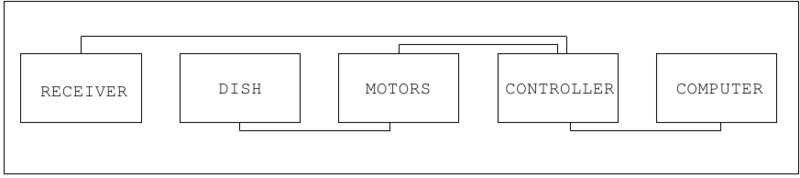
\includegraphics[width=0.4\textwidth]{block}
  \caption{A block diagram of our computer interface and its communication with our telescope. The computer ultimately controls motors on the telescope, which allow for position adjustement. A receiver processes our collected data and then sends it back to the computer.}
\end{figure}
Using a noise diode attached to the SRT, we are able to calibrate our apparatus in order to account for both external sources of radiation in the sky and noise generated by the antenna. Correcting our data due to external sources is done automatically through the SRT software, whereas the noise generated by the antenna - the \textit{antenna temperature} - is given by the software as a value which must be manually subtracted from our data.

\subsection{Sun Calibration}
\begin{figure}
  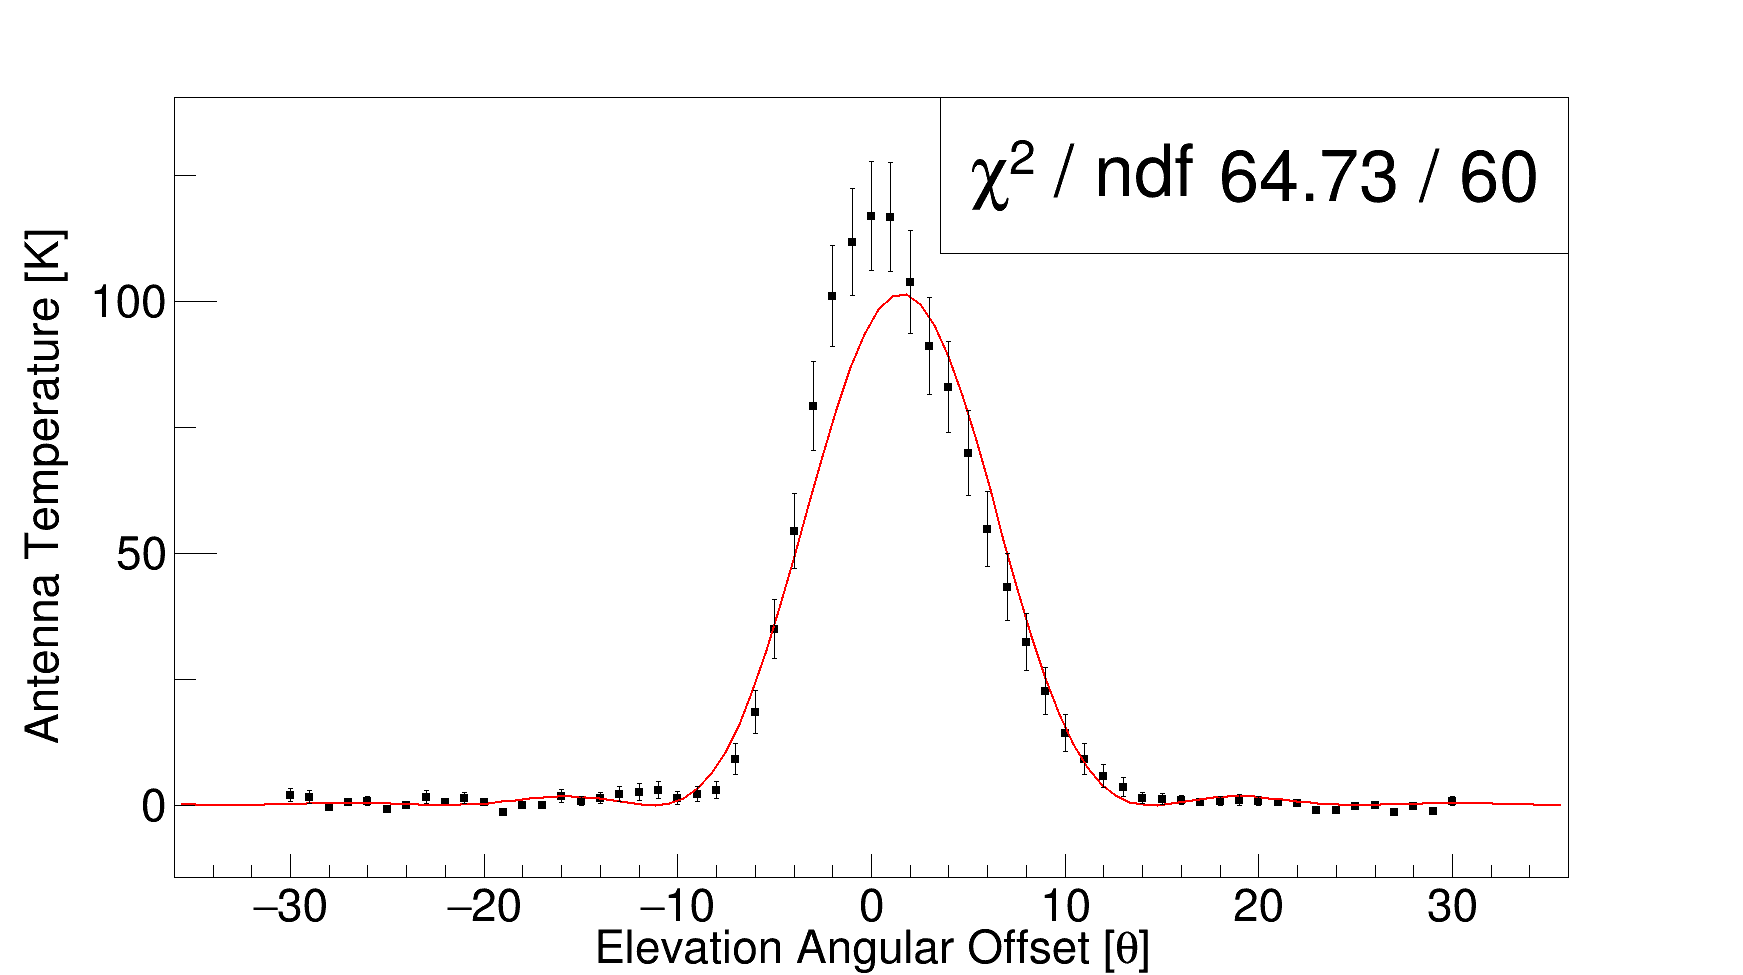
\includegraphics[width=0.5\textwidth]{elevation} 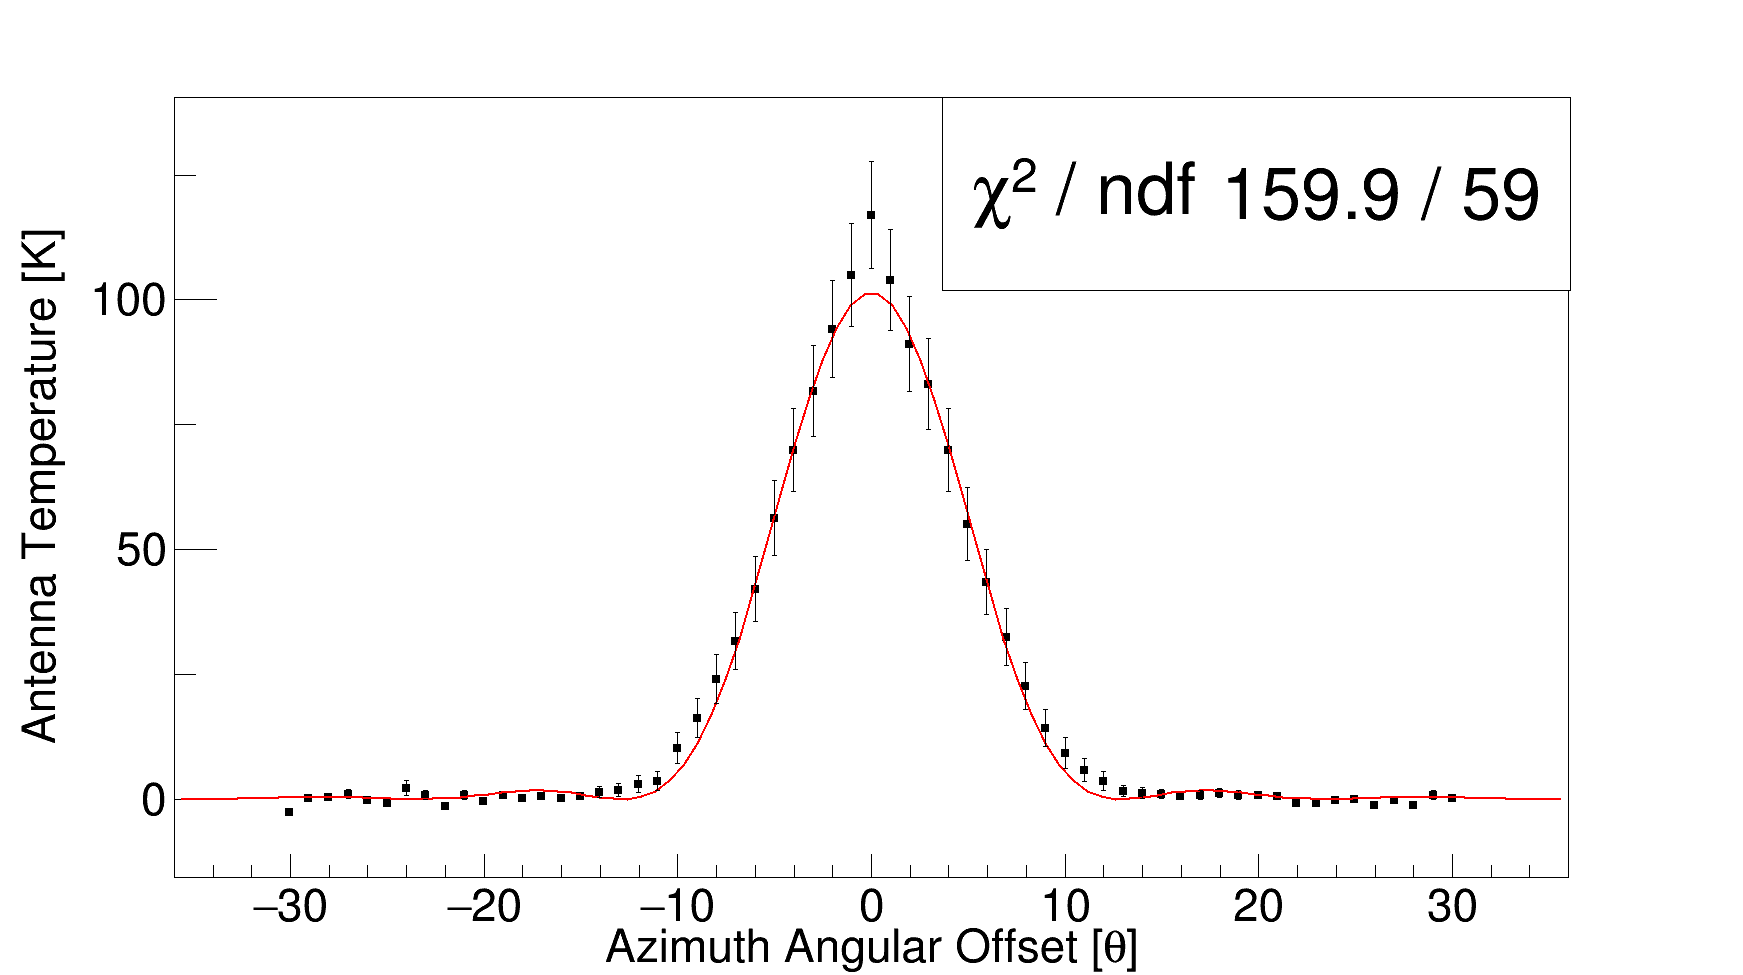
\includegraphics[width=0.5\textwidth]{azimuth_large}
  \caption{The antenna temperature as a function of elevation and azimuth angular offset from the sun. The theoretical antenna pattern described by equation $(3)$ is fitted to both these graphs. The top graph and fit is off center by $1.5\degree$, indicating a slight calibration error in our SRT.}
\end{figure}

\subsection{Data Collection}
The SRT software is able to determine the configuration corresponding to pointing our SRT dish along the plane of our galaxy at an angle $\ell$ from the center of the galaxy. Using this, we collect data from $90\degree \leq \ell \leq 180\degree$ in five degree increments. As our beam width is approximately seven degrees, taking data in increments significantly less than this is does not allow for increased resolution. At each angle, our telescope records data for approximately five seconds. In order to reduce statistical fluctuations and increase accuracy, we take fifty measurments at each angle and average them together.
\begin{figure}
  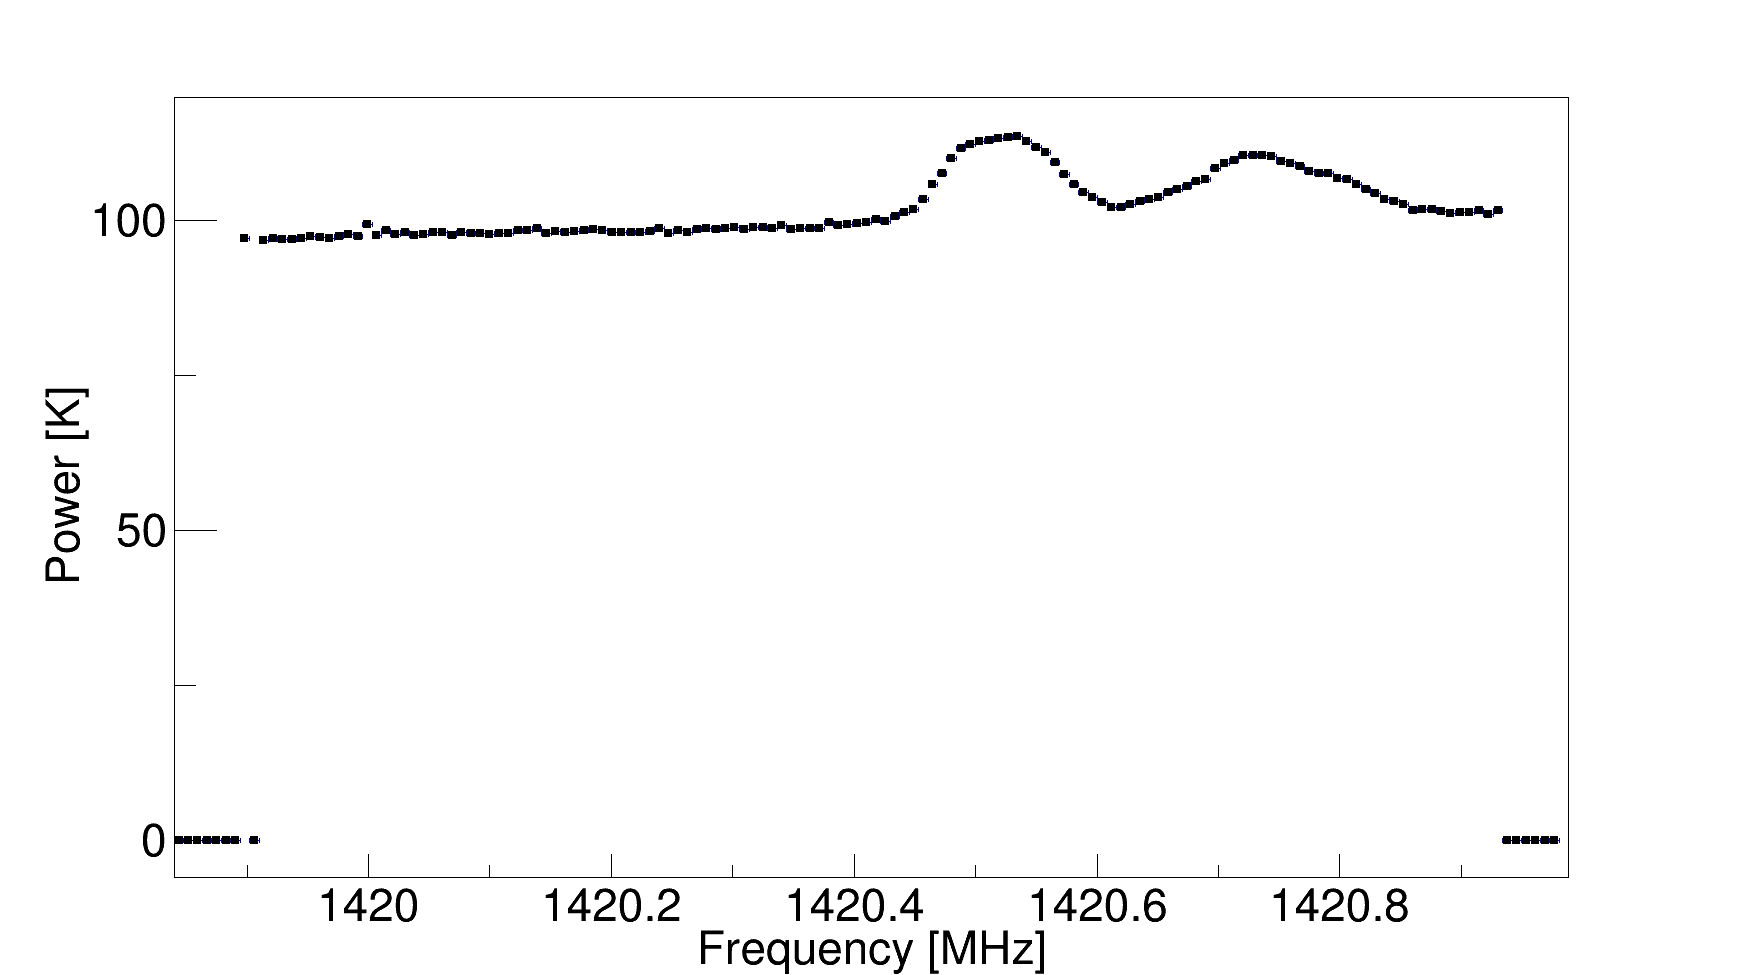
\includegraphics[width=0.5\textwidth]{data}
  \caption{The raw data received from our SRT Telescope at $\ell=115\degree$, averaged over 50 runs. The antenna temperature of 97 K must be subtracted to acquire the data of interest. In each individual run, every point has a Poissonian uncertainty associated with it. Averaging over fifty runs gives uncertainties on each point bewteen $0.25$ and $0.75$, which are too small to observe at this scale.}
  \label{raw}
\end{figure}
An example readout from our SRT, averaged over 50 runs, is displayed in Figure \ref{raw}. Most notably are two peaks in the brightness temperature to the right of the $1420.4$ MHz line, which we expect to correspond to two different concentrations of hydrogen at two different velocities.

\section{Data Analysis}
\subsection{Anomolous Data}
Upon collecting our data and subtracting out the antenna temperature, we are able to map the frequency of each data point to a velocity, and then by using the velocity along with the observation angle $\ell$, map this to a point in our galaxy corresponding to a density proportional to the brightness temperature measured multiplied by $r$, the distance from our sun to the hydrogen source \footnote{The power emitted from our sources falls off as $1/r^2$, so this factor must be taken into account to determine the density. However, the area of the bins we use to represent our data grow proprotional to $r$, so we ultimately only multiply by one factor of $r$.}. Before doing this, we examine our data taken for anomolous points. These correspond to sharp peaks in our data, usually over the span of a single or handful of points. As we expect any radiation from galactic sources to have some spread due to spectral broadening (detailed later), we suspect these points either correspond to a terrestrial source unaccounted for by the calibration, or from an internal error in the telescope - potentially due to the stitching together of multiple measurements. As these points do not come from galactic hydrogen, we remove them from our data.

\begin{figure}
  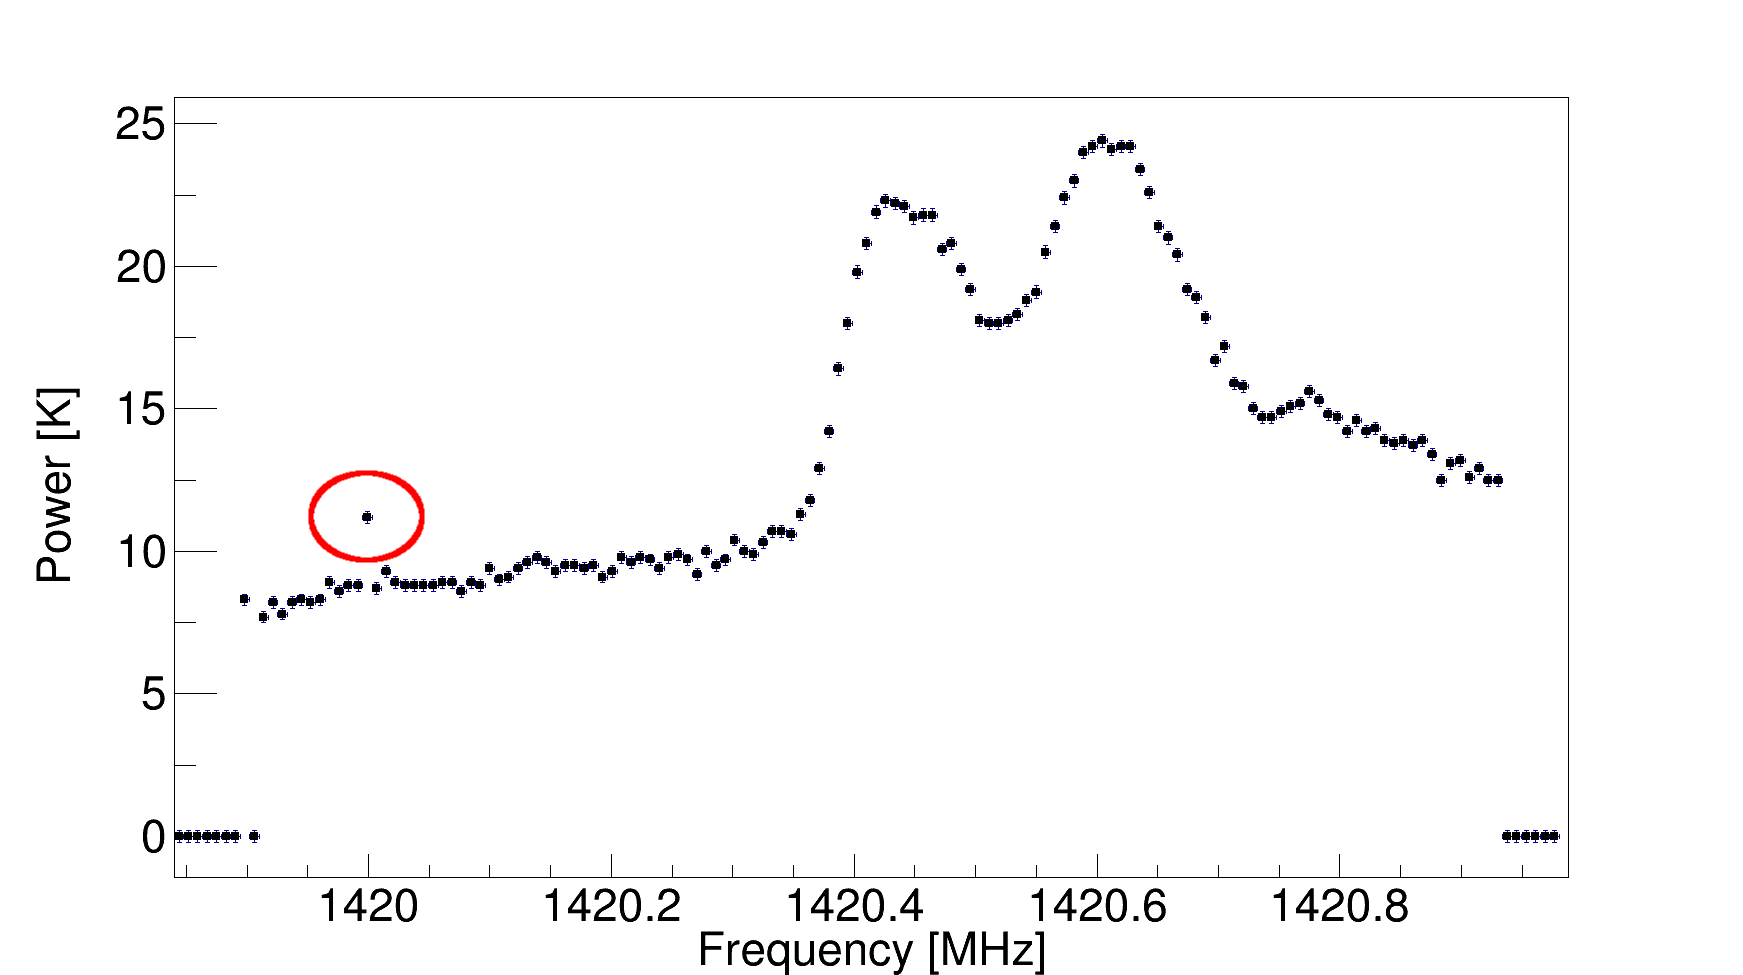
\includegraphics[width=0.5\textwidth]{anomolous}
  \caption{An example of data taken at $\ell=140\degree$. The antenna temperature of 97 K has been subtracted from the data. Circled in red is the anomolous point, which we hypothesize either comes from a terrestrial source unaccounted for by the calibration, or from some internal error in the telescope.}
\end{figure}

\subsection{Spectral Broadening}
We expect the emission lines from galactic sources to be spread out due to thermal effects. While a large mass of hydrogen will move at some average velocity relative to the center of the galaxy, the individual atoms can move around inside the large mass due to the non-zero temperature of our galaxy. We measure this thermal broadening by analyzing data collected at $\ell=180\degree$. At this point, we expect any hydrogen to be stationary relative to our motion. However, as shown in Figure \ref{thermal}, this distribution is spread out due to thermal effects. The effects of thermal broadening are predicted to broaden spectral lines into a Gaussian shape \cite{thermal-spread}. As such, we fit to a Gaussian to determine a standard deviation of $12.97 \pm 0.07$ km/s. Considering a spreading of our data by $2\sigma$, we determine that this systematic "smearing" has the effect of spreading a source across a distance of between 0.5 and 1.3 kpc, depending on the observation angle. This puts a restriction on the radial resolution of our data, but still allows us to extract qualitative features of our galactic hydrogen density.

\begin{figure}
  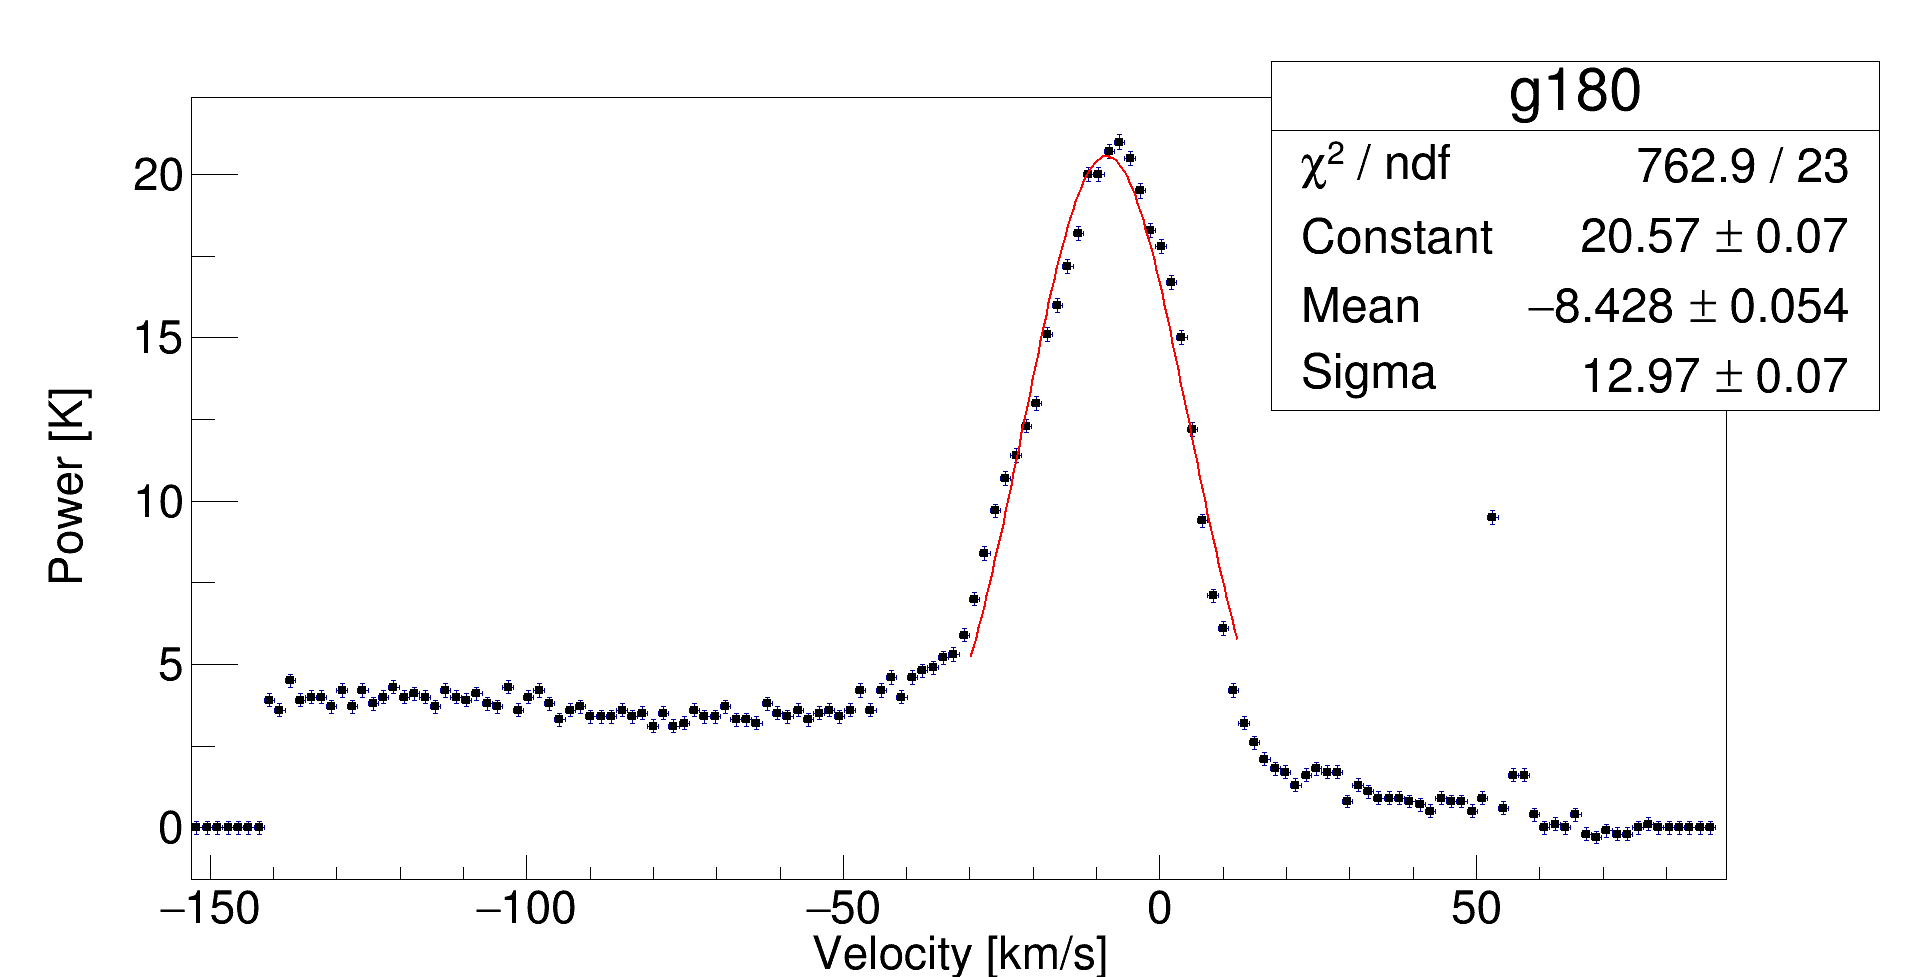
\includegraphics[width=0.5\textwidth]{thermal_large}
  \caption{The thermal broadening of the 21cm emission line at $\ell=180\degree$. This spread is fit to a Gaussian, which gives a $\sigma = 12.97 \pm 0.07$ km/s.}
  \label{thermal}
\end{figure}

\subsection{Uncertain Galactic Constants}

In order to analyze our data, we require the velocity of the sun and the distance from the sun to the center of the galaxy. Both of these constants are uncertain, with the former reported as $8.2 \pm 0.5$ kpc, and the latter as $223 \pm 17$ km/s. This contributes to uncertainty in our results, but only as a matter of scale. Variations in these constants change the overall length scale of the hydrogen density map, but do not noticiably impact the structure of the map. As such, we expect that the hydrogen density map that we acquire may vary in size from other hydrogen density maps constructed in other sources.

\section{Results and Discussion}
After mapping our data to a polar histogram, we acquire a mapping of the density of neutral hydrogen in the galaxy, displayed in Figure \ref{result}. Only the \textit{relative} densities of neutral hydrogen are mapped. A calculation of the actual densities of neutral hydrogen would require calculating the brightness temperature detected from a single hydrogen hyperfine transition, as well as the probability of these transitions occuring within the time of our data collection. Further theoretical considerations would be necessary to determine how the brightness temperature measured corresponds to the density of neutral hydrogen that has already undergone its hyperfine transition and decayed to its lowest energy state.

The relative densities of hydrogen still allow us to extract information about the structure of the Milky Way. Seen between $95 \leq \ell \leq 140$ are two separate concentrations of hydrogen densities, although the distinction between the two is diminished by thermal broadening. By comparing to a density map calculated by Westerhout \cite{wester}, as shown in Figure \ref{comp}, we see that these two densities correspond to the Orion and Perseus spiral arms of our galaxy. A rescaling of Westerhout's axes are necessary for it to agree with our data - as previously mentioned, this can be attributed to different constants used in calculations.

\begin{figure}
  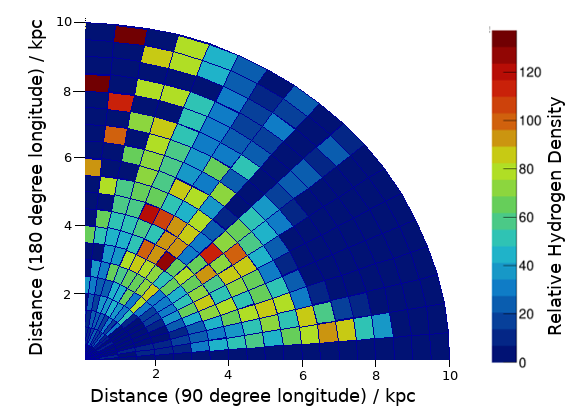
\includegraphics[width=0.5\textwidth]{final}
  \caption{A hydrogen densitiy map of a portion of our galaxy, calculated from the data acquired by calculating the sources of our 21cm emissions via Doppler analysis. The sun is located at the (0,0) point. }
  \label{result}
\end{figure}

\begin{figure}
  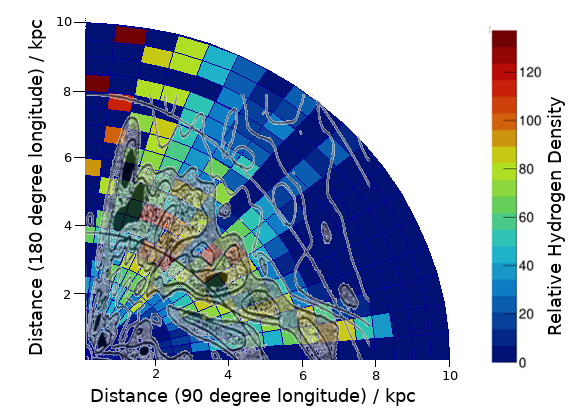
\includegraphics[width=0.5\textwidth]{final_wester}
  \caption{Our calculated hydrogen density map compared with a hydrogen density map determined by Westerhout \cite{westerhout}. After a rescaling of axis, the two plots show general agreement on galactic structure.}
  \label{comp}
\end{figure}

\end{document}
